%%%%%%%%%%%%%%%%%%%%%%%%%%%%%%%%%%%%%%%%%%%%%%%%%%%%%%%%%%%%%%%%%%%%%%
% LaTeX Example: Project Report
%
% Source: http://www.howtotex.com
%
% Feel free to distribute this example, but please keep the referral
% to howtotex.com
% Date: March 2018
% 
%%%%%%%%%%%%%%%%%%%%%%%%%%%%%%%%%%%%%%%%%%%%%%%%%%%%%%%%%%%%%%%%%%%%%%
% How to use writeLaTeX: 
%
% You edit the source code here on the left, and the preview on the
% right shows you the result within a few seconds.
%
% Bookmark this page and share the URL with your co-authors. They can
% edit at the same time!
%
% You can upload figures, bibliographies, custom classes and
% styles using the files menu.
%
% If you're new to LaTeX, the wikibook is a great place to start:
% http://en.wikibooks.org/wiki/LaTeX
%
%%%%%%%%%%%%%%%%%%%%%%%%%%%%%%%%%%%%%%%%%%%%%%%%%%%%%%%%%%%%%%%%%%%%%%
% Edit the title below to update the display in My Documents
%\title{Project Report}
%
%%% Preamble
\documentclass[paper=a4, fontsize=11pt]{scrartcl}
\usepackage[T1]{fontenc}
\usepackage{fourier}

\usepackage[english]{babel}                                                                                                                     % English language/hyphenation
\usepackage[protrusion=true,expansion=true]{microtype}  
\usepackage{amsmath,amsfonts,amsthm} % Math packages
\newcommand*{\rttensor}[1]{\overline{\overline{#1}}}
\newcommand{\pfrac}[2]{\frac{\partial#1}{\partial#2}}

\usepackage[pdftex]{graphicx}  

\usepackage{listings}

\usepackage{url}


\usepackage[numbers]{natbib}
%\usepackage[style=ieee]{biblatex}

%%% Custom sectioning

\usepackage{sectsty}
\allsectionsfont{\centering \normalfont\scshape}


%%% Custom headers/footers (fancyhdr package)
\usepackage{fancyhdr}
\pagestyle{fancyplain}    
\fancyhead{}% No page header
\fancyfoot[L]{}% Empty 
\fancyfoot[C]{}% Empty
\fancyfoot[R]{\thepage}% Pagenumbering
\renewcommand{\headrulewidth}{0pt}% Remove header underlines
\renewcommand{\footrulewidth}{0pt}% Remove footer underlines
\setlength{\headheight}{10.6pt}


%%% Equation and float numbering
\numberwithin{equation}{section}                % Equationnumbering: section.eq#
\numberwithin{figure}{section}                  % Figurenumbering: section.fig#
\numberwithin{table}{section}                           % Tablenumbering: section.tab#


%%% Maketitle metadata
\newcommand{\horrule}[1]{\rule{\linewidth}{#1}}         % Horizontal rule

\title{%\vspace{-1in}      
    \usefont{OT1}{bch}{b}{n}
    \normalfont\normalsize \textsc{Kevin T. Crofton Department of Aerospace and Ocean Engineering} \\ [25pt]
    \horrule{0.5pt} \\[0.4cm]
    \huge Magneto Rayleigh-Taylor Instability for an Annulus using Finite Volume Method with the MagnetoHydroDynamic Equations  \\
    \horrule{2pt} \\[0.5cm]}
\author{\normalfont\normalsize
  Robert Masti\\[-3pt]  
  \normalsize\today}
\date{}


%%% Begin document
\begin{document}
\maketitle
\section{MRT Overview \& Simulation Setup}\label{sec:ovrvw}
The magneto Rayleigh-Taylor instability (MRT) occurs when there is a heavy fluid supported by a light fluid under the influence of gravity with the addition of magnetic fields. Depending on the orientation of these magnetic fields they can have stabilizing characteristics for the growth of this instability. MRT is a hydrodynamic instability so it can be modeled using the ideal MagnetoHydroDynamic (MHD) equations. This instability is one of the most detrimental instabilities in the plasma communities attempt to reach fusion ignition. Specifically as it applies to inertial confinement fusion devices such as the one at NIF in the Direct Drive concept shown in Figure


  \begin{figure}[!htb]
    \centering
    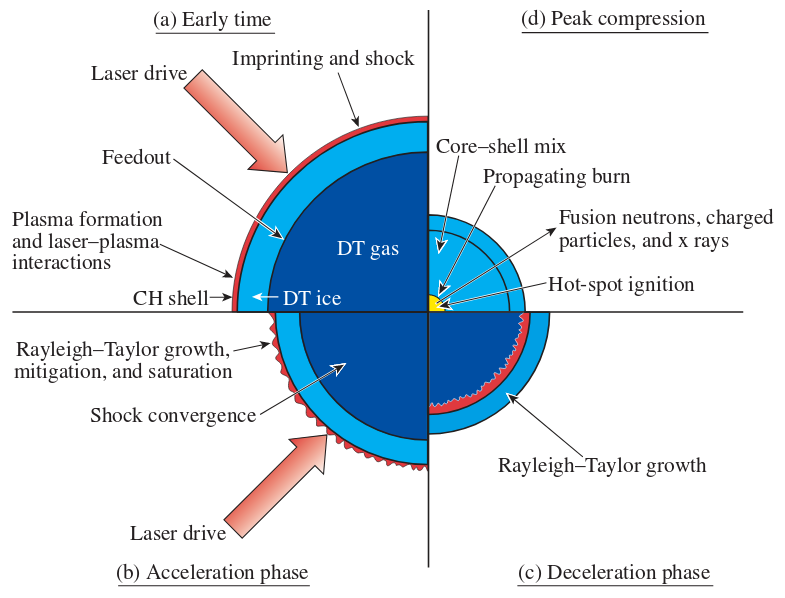
\includegraphics[width=0.9\linewidth]{fig/DDfusion}\label{fig:ovrvw:dd}
    \caption{Shows the four main stages during a typical direct-drive target implosion.\cite{craxton2015}}
  \end{figure}
 



\subsection{MHD Equation System}

The MHD equations are given by

\minipage{\textwidth}
  \minipage{0.48\textwidth}
  \begin{align*}
    \pfrac{\rho}{t} + \nabla \cdot \left[\rho \mathbf{u}\right] &= 0 \\
    \pfrac{\rho \mathbf{u}}{t} + \nabla \cdot \left[\rho \mathbf{u}\mathbf{u}^T - \mathbf{b}\mathbf{b}^T + \mathbb{I}\left(P + \frac{1}{2}|\mathbf{b}|^2\right)\right] &= 0 \\
    \pfrac{\epsilon}{t} + \nabla \cdot \left[\left(\epsilon + P + \frac{1}{2}|\mathbf{b}|^2\right)\mathbf{u}- \mathbf{b}\cdot\mathbf{u}\mathbf{b}\right] &= 0 \\
    \pfrac{\mathbf{b}}{t} + \nabla\times\mathbf{e} &= 0 \\
  \end{align*}
  \endminipage\hfill
  \minipage{0.48\textwidth}
  \begin{align*}
    \mathbf{b} &= \frac{\mathbf{B}}{\sqrt{\mu_0}} \\
    \mathbf{e} &= - \mathbf{u} \times \mathbf{b} +\left(\mathbf{e}^{external}\rightarrow\mathbf{0}\right)\\
    \epsilon &= \epsilon_{internal} + \frac{1}{2}\rho|\mathbf{u}|^2 + \frac{1}{2}|\mathbf{b}|^2\\
    P &=\rho \epsilon_{internal} (\gamma - 1) \\
  \end{align*}
  \endminipage\hfill
  \endminipage, where the ideal gas is assumed and there is no external electric fields ($e.q.\;\eta \mathbf{j}$). The equation for the magnetic field must be manipulated with vector identities into a divergence form through
  \begin{align*}
    \pfrac{\mathbf{b}}{t} + \nabla\times(-\mathbf{u}\times\mathbf{b}) &= 0\\
    \pfrac{\mathbf{b}}{t} - \left[\mathbf{u}(\nabla\cdot\mathbf{b})-\mathbf{b}(\nabla\cdot\mathbf{u})+(\mathbf{b}\cdot \nabla)\mathbf{u}-(\mathbf{u}\cdot\nabla)\mathbf{b}\right] &= 0\\
    \pfrac{\mathbf{b}}{t} - \left[\nabla\cdot(\mathbf{b}\mathbf{u}^T)-\nabla\cdot(\mathbf{u}\mathbf{b}^T)\right] &= 0\\
    \pfrac{\mathbf{b}}{t} + \nabla\cdot\left[\mathbf{u}\mathbf{b}^T-\mathbf{b}\mathbf{u}^T\right] &= 0\\
  \end{align*}, and it now is in divergence form which can be used to write into the tensor product form.


The conservative variable are density, momentum, total energy, and magnetic field. For the given problem however it is more convenient to rewrite as
\begin{equation}\label{eqn:mhdvector}
  \pfrac{\mathbf{Q}}{t} + \nabla \cdot \rttensor{T} = 0
\end{equation}
where $\mathbf{Q}$ is the conserved variables vector, and $\rttensor{T}$ is the flux tensor. Where the conserved variables vector, and flux tensor, are given by
\[
  \mathbf{Q}=
  \begin{bmatrix}
    \rho  \\
    \rho \mathbf{u}  \\
    \epsilon\\
    \mathbf{b} 
  \end{bmatrix}
  ,\quad \rttensor{T} =
  \begin{bmatrix}
    \rho \mathbf{u}  \\
    \rho \mathbf{u}\mathbf{u}^T - \mathbf{b}\mathbf{b}^T + \mathbb{I}\left(P + \frac{1}{2}|\mathbf{b}|^2\right)\\
    \left(\epsilon + P + \frac{1}{2}|\mathbf{b}|^2\right)\mathbf{u}- \mathbf{b}\cdot\mathbf{u}\mathbf{b}\\
    \mathbf{u}\mathbf{b}^T-\mathbf{b}\mathbf{u}^T
  \end{bmatrix}
\]
, respectively. 
  
  Phasellus viverra nulla ut metus varius laoreet. Quisque rutrum. Aenean imperdiet. Etiam ultricies nisi vel augue. Curabitur ullamcorper ultricies 

\subsection{Disc}
In 2D Cartesian coordinates equation~\ref{eqn:mhdvector} can be rewritten as 
\begin{equation} \label{eqn:mhdvecflux}
  \pfrac{\vec{Q}}{t} + \pfrac{\vec{F}}{x} + \pfrac{\vec{G}}{y} = 0
\end{equation}
where $\vec{F}$ is the $\hat{x}$ direction flux, and $\vec{G}$ is the $\hat{y}$ direction flux. Expanding the flux tensor through evaluating the dyadic terms, and collecting non-zero unit vectors $\vec{F}$, and $\vec{G}$ can be easily found. Equation~\ref{eqn:mhdvecflux} can be expanded into  
\[
  \pfrac{}{t}
  \begin{bmatrix}
    \rho  \\
    \rho u  \\
    \rho v \\
    \rho w \\
    B_x \\
    B_y \\
    B_z \\
    \epsilon
  \end{bmatrix}
  \;+\;\pfrac{}{x}
  \begin{bmatrix}
    \rho u  \\
    \rho u^2 + P + \frac{B^2}{2 \mu_0} - \frac{B_x^2}{\mu_0} \\
    \rho u v - \frac{B_x B_y}{\mu_0} \\
    \rho u w - \frac{B_x B_z}{\mu_0} \\
    0 \\
    B_y u - B_x v \\
    B_z u - B_x w \\
    \left(\epsilon+ P + \frac{B^2}{2 \mu_0} \right) u - B_x\frac{\vec{u}^T\cdot\vec{B}}{\mu_0}
  \end{bmatrix}
  \;+\;\pfrac{}{y}
  \begin{bmatrix}
    \rho v  \\
    \rho v u - \frac{B_y B_x}{\mu_0} \\
    \rho v^2 + p + \frac{B^2}{2 \mu_0} - \frac{B_y^2}{\mu_0} \\
    \rho v w - \frac{B_y B_z}{\mu_0} \\
    B_x v - B_y u \\
    0 \\
    B_z v - B_y w \\
    \left(\epsilon+ P + \frac{B^2}{2 \mu_0} \right) v - B_y\frac{\vec{u}^T\cdot\vec{B}}{\mu_0}
  \end{bmatrix}
  =0
\]





\begin{align}
  A = 
  \begin{bmatrix}
  A_{11} & A_{21} \\
    A_{21} & A_{22}
  \end{bmatrix}
\end{align}
Aenean commodo ligula eget dolor. Aenean massa. Cum sociis natoque penatibus et magnis dis parturient montes, nascetur ridiculus mus. Donec quam felis, ultricies nec, pellentesque eu, pretium quis, sem.

\subsubsection{Heading on level 3 (subsubsection)}
Nulla consequat massa quis enim. Donec pede justo, fringilla vel, aliquet nec, vulputate eget, arcu. In enim justo, rhoncus ut, imperdiet a, venenatis vitae, justo. Nullam dictum felis eu pede mollis pretium. Integer tincidunt. Cras dapibus. Vivamus elementum semper nisi. Aenean vulputate eleifend tellus. Aenean leo ligula, porttitor eu, consequat vitae, eleifend ac, enim.

\paragraph{Heading on level 4 (paragraph)}
Lorem ipsum dolor sit amet, consectetuer adipiscing elit. Aenean commodo ligula eget dolor. Aenean massa. Cum sociis natoque penatibus et magnis dis parturient montes, nascetur ridiculus mus. Donec quam felis, ultricies nec, pellentesque eu, pretium quis, sem. Nulla consequat massa quis enim. 


\begin{lstlisting}
int a = 4;
\end{lstlisting}

\section{Lists}

\subsection{Example for list (3*itemize)}
\begin{itemize}
  \item First item in a list 
    \begin{itemize}
    \item First item in a list 
      \begin{itemize}
      \item First item in a list 
      \item Second item in a list 
      \end{itemize}
    \item Second item in a list 
    \end{itemize}
  \item Second item in a list 
\end{itemize}

\subsection{Example for list (enumerate)}
\begin{enumerate}
  \item First item in a list 
  \item Second item in a list 
  \item Third item in a list
\end{enumerate}
\cite{Slutz2010}
 \bibliographystyle{IEEEtran}
  \bibliography{reference}
%%% End document
\end{document}
